% Q1-sim：问题一修改后章节（供论文手直接并入 main.tex）
% 修改内容：模型准备三块合一；结果解读删除铺垫与重复校验句、图注压缩；小结压缩。
% 图表与公式均未改动（图宽、表内容与原版一致）；校验细节以第八章为准。
% 问题一
\section{问题一的模型建立与求解}

\subsection{模型准备}

本问数据为附件 1 与附件 2：附件 1 提供 6 个蔬菜品类、251 个单品（246 个有售）的标识信息；附件 2 为 2020-07-01 至 2023-06-30 的销售流水，共 878,503 行，其中退货 461 行按负销量并入当日净销量口径。按“日期$\times$单品”将流水聚合为单品日销量表（46,599 行），再按品类汇总为品类日销量表（6,474 行）；以完整日历（$T=1095$ 天）为基准补零对齐各序列，供季节分解、残差回归与特征计算使用。数据预处理代码见附录\ref{clean_data}。

\subsection{模型建立}

\subsubsection{品类与单品销量分布模型}

品类日销量为连续正值、右偏长尾，选用对数正态分布（lognormal）与伽马分布（gamma）两类连续分布拟合，并以 AIC\cite{akaike1974}/BIC\cite{schwarz1978} 选型。两类分布均固定位置参数 $\mathrm{loc}=0$，使支撑为 $(0,\infty)$，与销量下界为 0 相符；固定位置参数亦避免无意义的平移外推。两类分布自由参数个数相同（均为 2），AIC/BIC 可直接比较。

对数正态分布：若 $\ln X \sim N(\mu, s^2)$，则 $X\sim\mathrm{LogNormal}(s,0,\mathrm{scale})$，其密度函数为
\begin{equation}\label{eq:lognorm}
  f(x)=\frac{1}{x\,s\sqrt{2\pi}}\exp\left(-\frac{(\ln x-\mu)^2}{2s^2}\right),\quad x>0
\end{equation}
其中 $s$ 为对数标准差，$\mathrm{scale}=e^\mu$ 为尺度参数，且 $E[X]=\mathrm{scale}\cdot e^{s^2/2}$，$\mathrm{Var}(X)=\mathrm{scale}^2(e^{s^2}-1)e^{s^2}$。

伽马分布：固定 $\mathrm{loc}=0$，记为 $X\sim\mathrm{Gamma}(a,0,\mathrm{scale})$，其密度函数为
\begin{equation}\label{eq:gamma}
  f(x)=\frac{x^{a-1}e^{-x/\mathrm{scale}}}{\Gamma(a)\,\mathrm{scale}^a},\quad x>0
\end{equation}
其中 $a$ 为形状参数，$\mathrm{scale}$ 为尺度参数，且 $E[X]=a\cdot\mathrm{scale}$，$\mathrm{Var}(X)=a\cdot\mathrm{scale}^2$。当 $a>1$ 时分布单峰右偏，$a$ 越大分布越集中。

设某品类正销量样本 $x_1,\dots,x_n$，密度函数为 $f(x;\theta)$，参数 $\theta$ 由最大似然估计得到：
\begin{equation}\label{eq:mle}
  L(\theta)=\prod_{i=1}^{n}f(x_i;\theta),\qquad
  \mathrm{LLF}=\ln L(\hat\theta)=\sum_{i=1}^{n}\ln f(x_i;\hat\theta)
\end{equation}
\begin{equation}\label{eq:aic}
  \mathrm{AIC}=2k-2\mathrm{LLF},\qquad
  \mathrm{BIC}=k\ln n-2\mathrm{LLF}
\end{equation}
其中 $k$ 为自由参数个数，$n$ 为正销量天数；AIC/BIC 取值越小表示模型越优，本文以 AIC 选型、BIC 交叉核对。拟合质量以 QQ 图诊断，以理论分位数与样本分位数的贴近程度检验分布假设。

单品日销量存在大量无销售日，采用两阶段模型\cite{mullahy1986}：令 $Y_t=\mathbf{1}\{q_t>0\}$ 表示第 $t$ 日是否销售，则 $Y_t\sim\mathrm{Bernoulli}(p_i)$，售出概率取经验频率 $p_i=n_i/T$；正销量条件分布 $q_t\mid Y_t=1\sim f(q;\theta_i)$ 按 AIC 在对数正态与伽马之间选优。单品日销量的整体分布为混合分布：
\begin{equation}\label{eq:mixture}
  f(q)=(1-p_i)\,\delta_0(q)+p_i\,f(q;\theta_i),\quad q\ge0
\end{equation}
其中 $\delta_0$ 为 0 点的点质量。对 $n_i<60$ 的稀疏单品不做参数估计，仅报告经验分位数 $Q_\tau=\inf\{x:F(x)\ge\tau\}$（$\tau=0.5,0.9,0.99$ 对应 P50、P90、P99），避免小样本下参数估计与分布外推不可靠。

\subsubsection{季节规律模型}

品类日销量受周内与年内规律共同驱动。周内规律体现为工作日与周末的需求差异，对应 7 天周期；年内规律受供给与需求季节性影响，但观测期仅 3 年、365 天周期循环数不足，直接估计年周期不稳定。本文采用 STL\cite{cleveland1990,hyndman2018} 对品类日销量做加性分解以刻画周季节，并对年季节改用月度聚合：
\begin{equation}\label{eq:stl}
  y_t = T_t + S_t + R_t
\end{equation}
其中 $T_t$ 为趋势项，$S_t$ 为季节项，$R_t$ 为残差项。STL 通过内层与外层循环迭代执行 loess 平滑估计各分量，对离群值具有鲁棒性。本文取季节周期 $\mathrm{period}=7$（周内季节）并启用 $\mathrm{robust}=True$，以降低极端促销日对分量估计的影响。

以方差分解度量季节与趋势成分的相对强度\cite{wang2006}：
\begin{equation}\label{eq:strength}
  F_s=\max\left(0,\;1-\frac{\mathrm{Var}(R_t)}{\mathrm{Var}(S_t+R_t)}\right),\qquad
  F_t=\max\left(0,\;1-\frac{\mathrm{Var}(R_t)}{\mathrm{Var}(T_t+R_t)}\right)
\end{equation}
$F_s$、$F_t\in[0,1]$，越接近 1 表示该成分对总波动的贡献越大。

年季节按月份聚合平均日销量 $\bar y_{c,m}$，定义旺季为 4-10 月、淡季为 11-3 月，旺季比值
\begin{equation}\label{eq:rho}
  \rho_c=\frac{\bar y_{c,\mathrm{peak}}}{\bar y_{c,\mathrm{off}}}
\end{equation}
$\rho_c>1$ 表示品类 $c$ 旺季平均日销量高于淡季。该指标用于检验题面"4-10 月供应丰富"的供给侧信息是否对应需求侧销量高峰。

\subsubsection{去季节协同变动网络模型}

单品日销量同时受日历效应与自身需求驱动，直接计算相关系数会产生由共同季节因素导致的伪相关\cite{yule1926,granger1974}，故先剔除日历效应。对每个单品 $i$ 拟合线性模型\cite{wooldridge2010}
\begin{equation}\label{eq:reg}
  q_{it}=\alpha_i+\sum_{k=1}^{6}\delta_k D^{\mathrm{wk}}_{kt}
  +\sum_{m=1}^{11}\eta_m D^{\mathrm{mo}}_{mt}+\varepsilon_{it}
\end{equation}
其中 $D^{\mathrm{wk}}_{kt}$、$D^{\mathrm{mo}}_{mt}$ 分别为星期与月份虚拟变量，参数由最小二乘估计；残差 $e_{it}=q_{it}-\hat q_{it}$ 为去日历效应后的销量序列。

对残差序列按日秩变换后取 Pearson 相关，得到 Spearman 秩相关系数\cite{spearman1904}
\begin{equation}\label{eq:spearman}
  r_{ij}=\mathrm{corr}\big(\mathrm{rank}(e_i),\,\mathrm{rank}(e_j)\big)
\end{equation}
秩相关对极端销量与分布形态不敏感，比 Pearson 相关更稳健。在原假设 $r_{ij}=0$ 下，检验统计量 $t=\dfrac{r_{ij}\sqrt{n-2}}{\sqrt{1-r_{ij}^2}}\sim t_{n-2}$，双侧 $p$ 值为 $p=2\big(1-F_t(|t|;n-2)\big)$。对全部 $m$ 个单品对的 $p$ 值做 BH-FDR 校正\cite{benjamini1995}：
\begin{equation}\label{eq:fdr}
  q_{(i)}=\min_{j\ge i}\left\{\frac{m}{j}p_{(j)}\right\}
\end{equation}
其中 $p_{(1)}\le\cdots\le p_{(m)}$ 为排序后的 $p$ 值。建边条件为 $|r_{ij}|\ge0.4$ 且 $q_{ij}<0.05$。随后将样本按时间分为前半（2020-07-01 至 2021-12-31）与后半（2022-01-01 至 2023-06-30），分别执行相同的残差化与秩相关检验，若某条边在两半中均满足 $p<0.05$ 且符号与全样本一致，则记为稳健边。前后半检验保证网络结构不依赖单一时段，避免将偶然相关误判为稳定关系。

以单品为节点、稳健边为边构建无向图\cite{tumminello2005,mantegna1999}，边权为相关系数，按符号区分正负相关；节点中心性采用度中心度与介数中心度\cite{freeman1977,wasserman1994}，用于识别销量协同变动中的关键单品。

\subsubsection{单品时序特征聚类模型}

不同单品在销售频率、销量水平、波动幅度与日历响应上差异悬殊，直接以原始序列聚类易受噪声与量纲干扰。本文对每个单品 $i$ 提取六维特征刻画其需求形态\cite{wang2006}：售出天数占比 $p_i$、有售日均销量 $\mu_i$、有售日变异系数 $\mathrm{CV}_i$、周末偏置 $w_i$、节假日脉冲 $h_i$ 与总销量占比 $s_i$，分别反映"多久卖一次、一次卖多少、波动多大、何时集中、节假日响应与体量贡献"：
\begin{equation}\label{eq:feat1}
  p_i=\frac{n_i}{T},\qquad
  \mu_i=\frac{1}{n_i}\sum_{q_{it}>0}q_{it},\qquad
  \mathrm{CV}_i=\frac{1}{\mu_i}\sqrt{\frac{1}{n_i}\sum_{q_{it}>0}(q_{it}-\mu_i)^2}
\end{equation}
\begin{equation}\label{eq:feat2}
  w_i=\frac{\bar q_{i,\mathrm{weekend}}}{\bar q_{i,\mathrm{weekday}}}-1,\qquad
  h_i=\frac{\bar q_{i,\mathrm{holiday}}}{\bar q_{i,\mathrm{other}}}-1,\qquad
  s_i=\frac{\sum_t q_{it}}{\sum_j\sum_t q_{jt}}
\end{equation}
其中均值均基于补零后的完整日序列计算，变异系数仅基于正销量样本以避免零值膨胀失真；节假日集合取中国法定节假日（含调休）。对六维特征做 z-score 标准化，消除量纲差异后计算欧式距离，采用 Ward 最小方差法层次聚类\cite{ward1963,murtagh2014,kaufman1990}，使簇内离差平方和最小、簇间差异最大；对 $k\in\{3,\dots,10\}$ 分别计算 silhouette 系数\cite{rouseeuw1987}，取 silhouette 最大且不小于 0.15 的 $k$ 为最优簇数。稳定性评估采用 80\% 抽样，重复聚类 50 次，以调整兰德指数（ARI）\cite{hubert1985} 度量抽样结果与全量聚类的一致性，取平均报告。

\subsection{模型求解与结果分析}

\subsubsection{分布拟合结果}

各品类正销量天数分别为 1085、1084、1085、1050、1085、1085，合计 6,474。AIC 选型结果：花叶类、花菜类、水生根茎类、茄类为伽马分布，辣椒类、食用菌为对数正态分布；AIC 与 BIC 选型完全一致，参数估计结果见表~\ref{tab:dist_cat}。

\begin{table}[htbp]
  \centering
  \caption{品类日销量的最优分布与 AIC/BIC}
  \label{tab:dist_cat}
  \begin{tabular}{lccccc}
    \toprule
    品类 & 最优分布 & 形状/对数标准差 & 尺度参数 & AIC & BIC \\
    \midrule
    花叶类 & gamma & 5.2599 & 34.8338 & 12444.912 & 12454.891 \\
    花菜类 & gamma & 2.9925 & 12.8900 & 9548.503 & 9558.480 \\
    水生根茎类 & gamma & 1.6376 & 22.8694 & 9898.119 & 9908.098 \\
    茄类 & gamma & 2.8055 & 7.6219 & 8059.611 & 8069.525 \\
    辣椒类 & lognorm & 0.5365 & 72.8523 & 11037.887 & 11047.866 \\
    食用菌 & lognorm & 0.6123 & 58.3107 & 10841.520 & 10851.499 \\
    \bottomrule
  \end{tabular}
\end{table}

伽马分布的形状参数揭示品类内部的集中程度：花叶类 $a=5.2599$，分布相对集中，说明日销量围绕均值波动较小；水生根茎类 $a=1.6376$，右偏更明显，存在更多高销量日。对数正态的形状参数 $s$ 刻画尾部厚度：辣椒类 $s=0.5365$ 尾部相对较薄，食用菌 $s=0.6123$ 略厚，说明食用菌出现极端高峰日的概率更高。

246 个有售单品中，132 个进入参数拟合（伽马 81 个、对数正态 51 个），114 个稀疏单品仅报告经验分位数，另有 5 个单品无销售记录。

图~\ref{fig:dist_qq} 的 QQ 图诊断显示各品类中部拟合良好、两端略有偏离，分布主体可由所选分布近似\cite{dagostino1986}。

\begin{figure}[htbp]
  \centering
  
\includegraphics[width=0.9\textwidth]{figures/q1_dist_cat_qq.pdf}
  \caption{品类日销量最优分布 QQ 图}
  \label{fig:dist_qq}
\end{figure}

\subsubsection{季节规律结果}

各品类季节强度介于 0.1729 至 0.2616，趋势强度介于 0.5135 至 0.6268，品类日销量以趋势成分为主、周季节成分中等偏弱；旺季检验结果见表~\ref{tab:season}。

\begin{table}[htbp]
  \centering
  \caption{品类季节强度、趋势强度与旺季检验结果}
  \label{tab:season}
  \begin{tabular}{lccccc}
    \toprule
    品类 & 季节强度 & 趋势强度 & 旺季平均日销量 & 淡季平均日销量 & 旺季比值 \\
    \midrule
    花叶类 & 0.2114 & 0.5518 & 188.110 & 171.871 & 1.0945 \\
    花菜类 & 0.2182 & 0.5135 & 38.311 & 37.975 & 1.0089 \\
    水生根茎类 & 0.1729 & 0.5389 & 30.206 & 46.748 & 0.6462 \\
    茄类 & 0.2385 & 0.6268 & 24.015 & 15.582 & 1.5412 \\
    辣椒类 & 0.2001 & 0.5174 & 78.951 & 90.792 & 0.8696 \\
    食用菌 & 0.2616 & 0.5729 & 56.150 & 88.527 & 0.6343 \\
    \bottomrule
  \end{tabular}
\end{table}

旺季比值超过 1 的品类为花叶类、花菜类与茄类；水生根茎类、辣椒类与食用菌淡季日销量反而更高。可见 4-10 月供给丰富并不必然对应销量高峰，问题二的定价与补货决策不能简单套用“旺季多备货”的经验规则。月度形态上，花叶类、花菜类、茄类在 7-8 月达年内高点，辣椒类、食用菌、水生根茎类在 1-2 月达年内高点。

\begin{figure}[htbp]
  \centering
  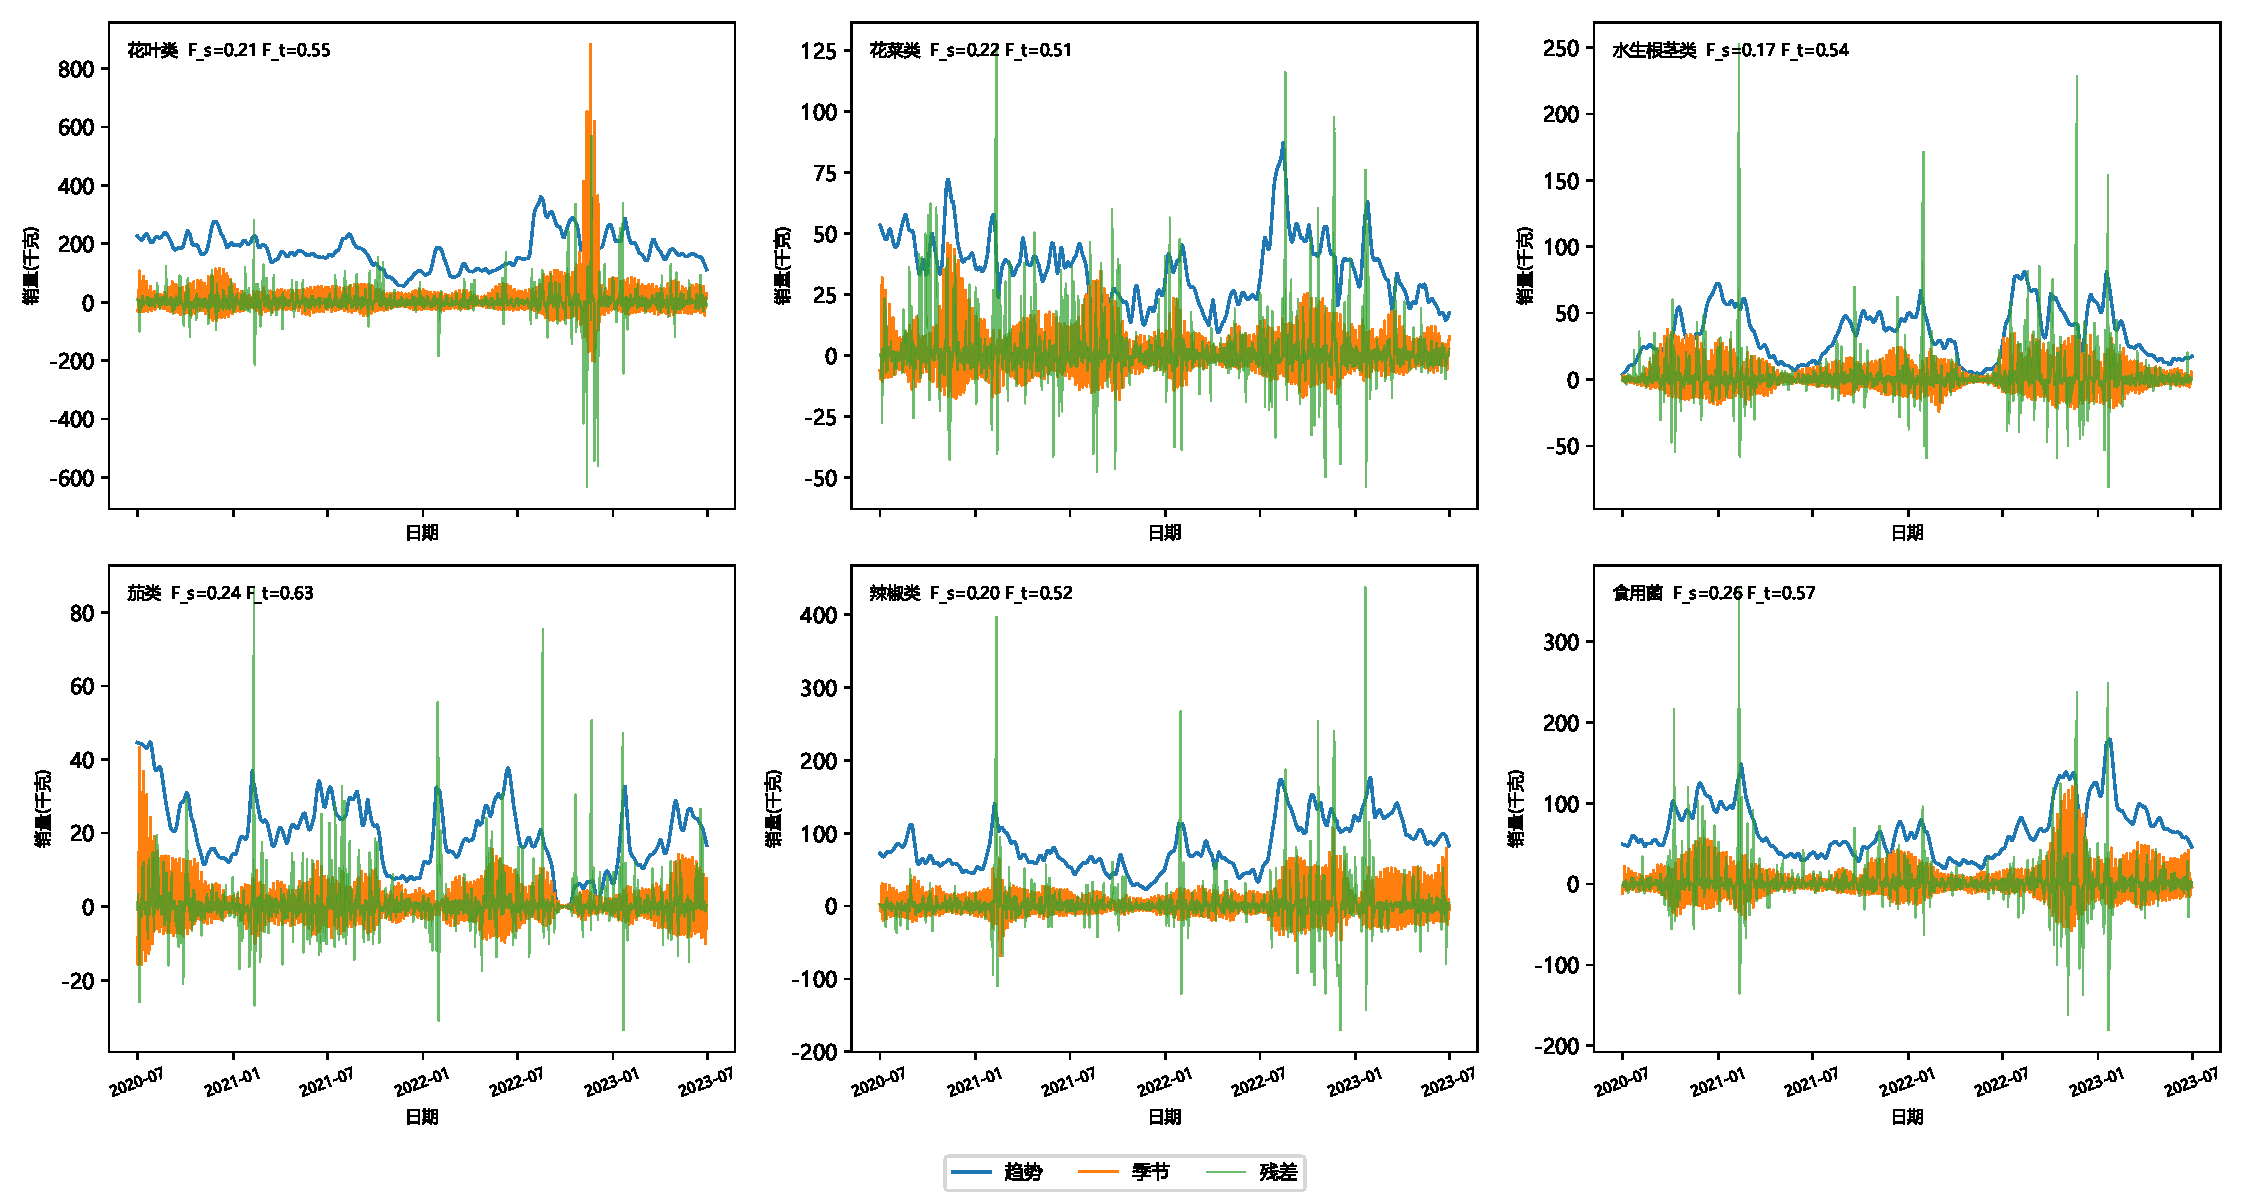
\includegraphics[width=0.95\textwidth]{figures/q1_stl.pdf}
  \caption{品类日销量 STL 分解图}
  \label{fig:stl}
\end{figure}

图~\ref{fig:stl} 显示季节分量呈明显周内起伏、残差围绕零波动。
\subsubsection{协同变动网络结果}

进入分析的 132 个单品共 8,646 个单品对。满足 $|r|\ge0.4$ 且 $q<0.05$ 的主边共 1,062 条，其中正相关 820 条、负相关 242 条；通过前后半样本检验的稳健边 154 条，构成包含 51 个节点的协同变动网络。相关系数阈值敏感性见表~\ref{tab:corr_thr}。

\begin{table}[H]
  \centering
  \caption{相关系数阈值敏感性分析}
  \label{tab:corr_thr}
  \begin{tabularx}{\textwidth}{c X c c c}
    \toprule
    阈值 & 边数统计 & 正边数 & 负边数 & 稳健边数 \\
    \midrule
    0.3 & 1848 & 1289 & 559 & 249 \\
    0.4 & 1062 & 820 & 242 & 154 \\
    0.5 & 523 & 456 & 67 & 81 \\
    \bottomrule
  \end{tabularx}
\end{table}

阈值从 0.3 提高到 0.5 时边数由 1848 降至 523，正边始终占多数，说明品类与单品销量以正向同步为主，负向关系仅存在于少数组合。品类级去季节残差的 Spearman 相关中，花叶类与食用菌、花叶类与辣椒类、辣椒类与食用菌相关较强（$|r|$ 约 0.64），茄类与其余品类相关最弱（$|r|<0.14$），在销量上相对独立。单品级网络中，度中心度最高的单品为红椒(1)、小米椒、青线椒等（中心度 0.3 以上），以正相关边为主。辣椒类、食用菌与花叶类单品之间呈现明显的正向同步变动，可作为销量同步变动的候选组合；是否构成需求互补，需结合问题二的交叉价格弹性进一步判定\cite{deaton1980,mascolel1995}。负相关边占比约 23\%（242/1062），可作为潜在替代关系候选。



图~\ref{fig:corr_net} 展示了按度中心度选取的 15 个代表性单品构成的协同变动网络（红色实线为正相关、蓝色虚线为负相关）。

\begin{figure}[htbp]
  \centering
  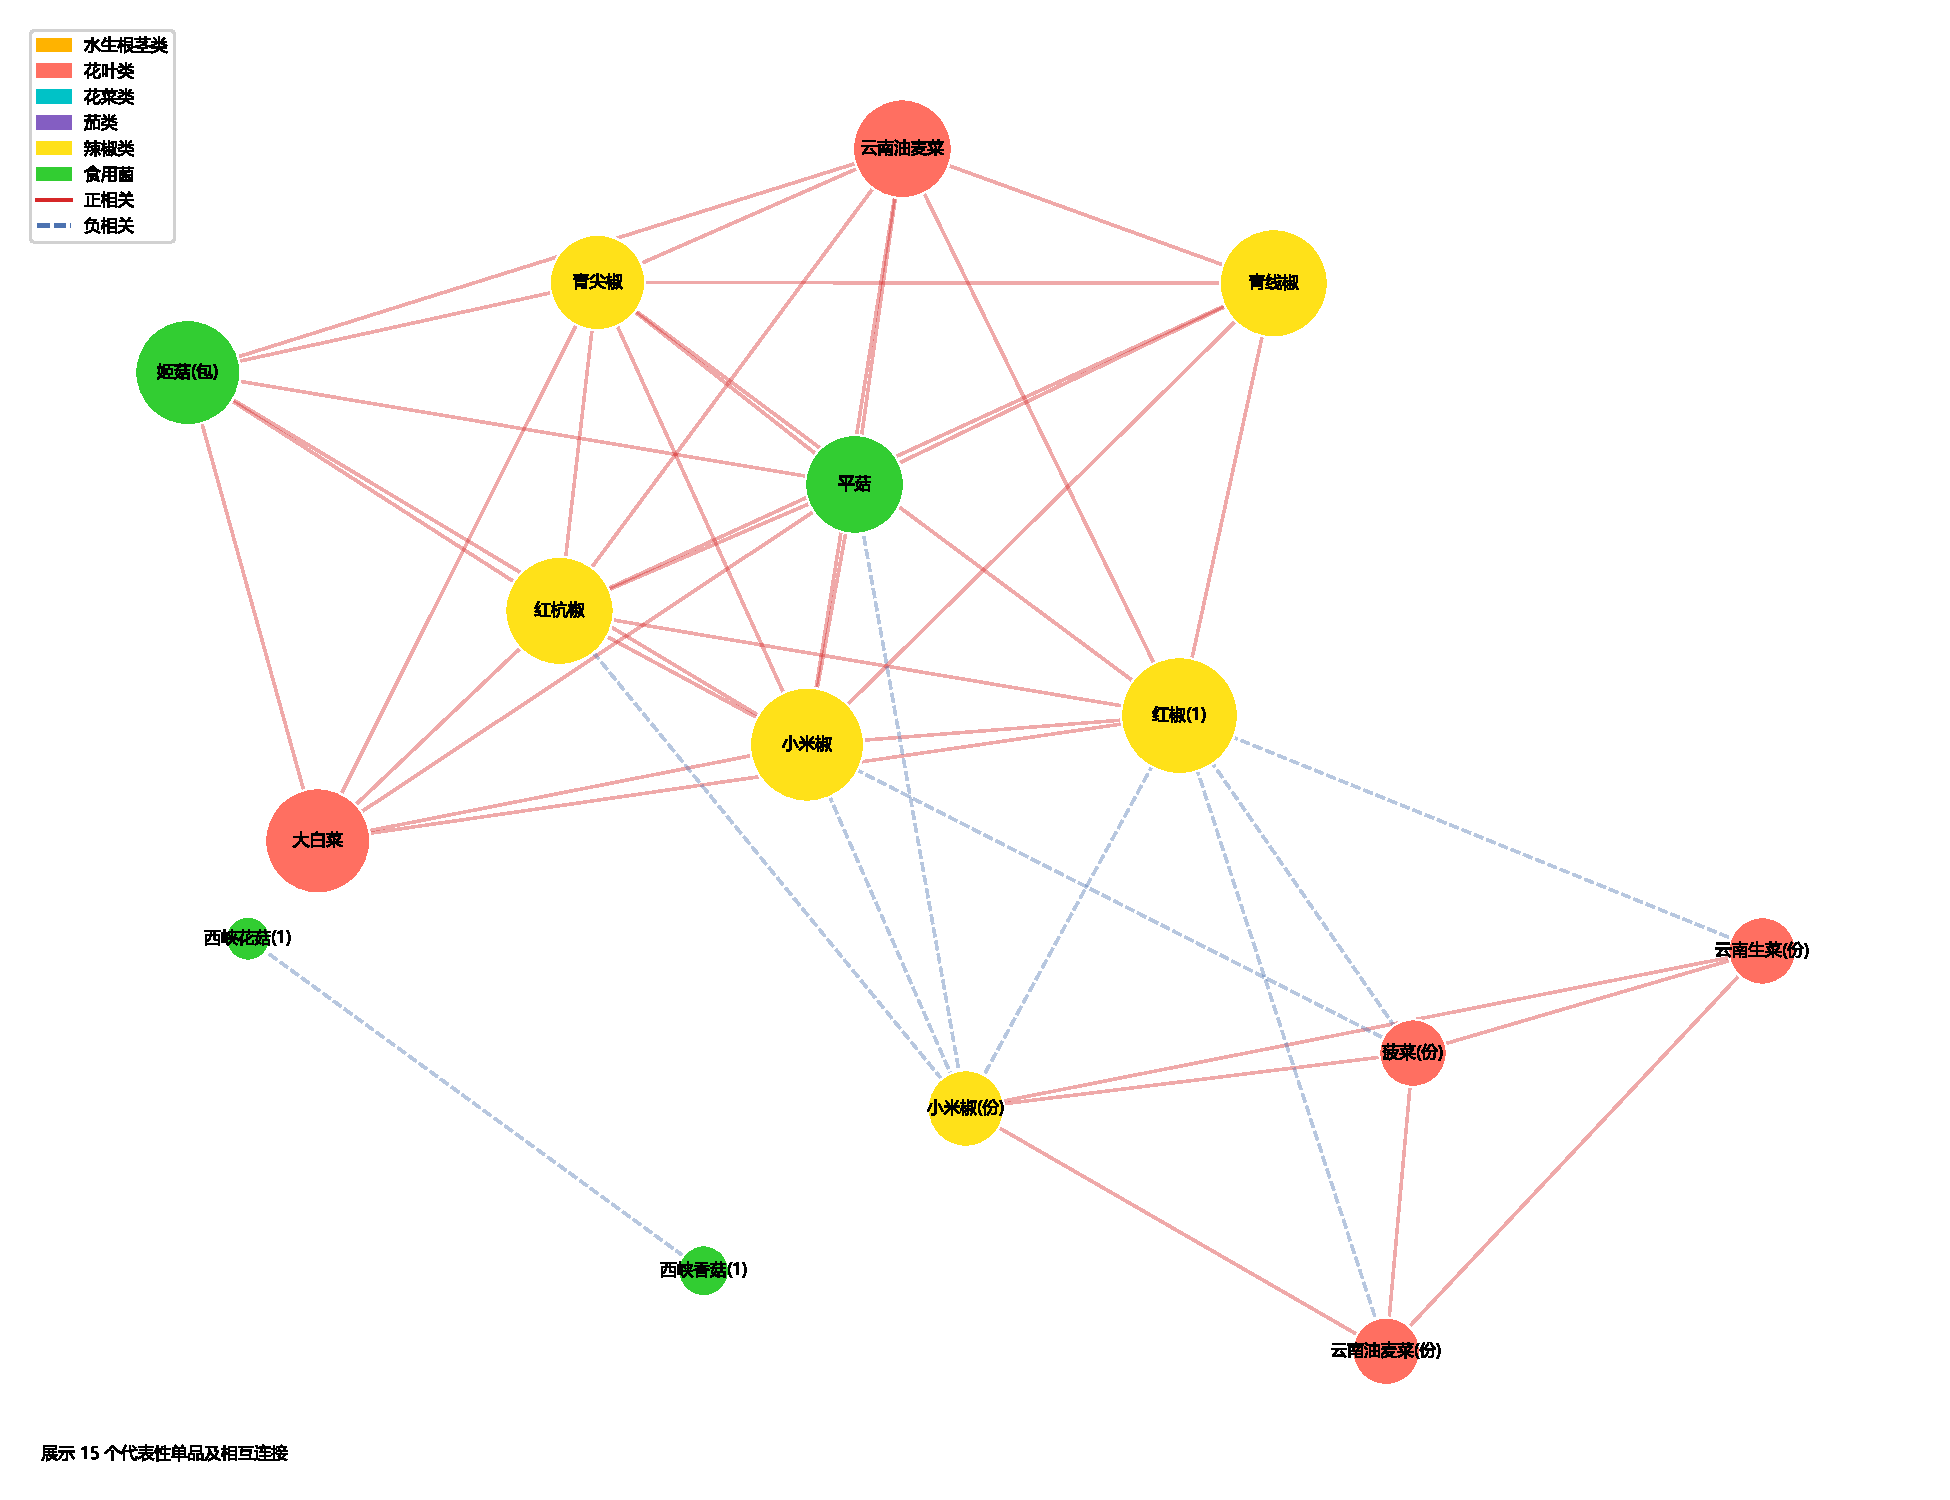
\includegraphics[width=0.9\textwidth]{figures/q1_corr_network.pdf}
  \caption{单品级协同变动网络}
  \label{fig:corr_net}
\end{figure}

\subsubsection{单品聚类结果}

132 个单品的最优簇数为 $k=5$，对应 silhouette 系数 0.2583；50 次 80\% 抽样聚类的平均 ARI 为 0.4567，聚类结构基本稳定。各簇画像见表~\ref{tab:cluster}。

\begin{table}[htbp]
  \centering
  \caption{单品聚类画像}
  \label{tab:cluster}
  \begin{tabular}{lcccccccc}
    \toprule
    簇 & 单品数 & 售出天数占比 & 有售日均销量 & 有售日变异系数 & 周末偏置 & 节假日脉冲 & 总销量占比 & 建议命名 \\
    \midrule
    1 & 13 & 0.3236 & 27.4374 & 0.6927 & 0.3466 & 0.3544 & 0.0207 & 高量周末脉冲型 \\
    2 & 7 & 0.8384 & 20.7024 & 0.7215 & 0.4876 & 0.5192 & 0.0414 & 高频平稳型 \\
    3 & 55 & 0.2053 & 4.7746 & 0.7616 & 0.2129 & 0.2126 & 0.0025 & 低频稀疏型 \\
    4 & 34 & 0.1908 & 6.1442 & 0.7681 & 0.5531 & 0.5963 & 0.0028 & 低频脉冲型 \\
    5 & 23 & 0.5631 & 7.3427 & 1.0807 & 0.3617 & 0.4005 & 0.0091 & 周末脉冲型 \\
    \bottomrule
  \end{tabular}
\end{table}

各簇特征差异明显：簇 1（高量周末脉冲型）呈“高量低频”特征，补货需预留较高单日峰值；簇 2（高频平稳型）适合作稳定的主销单品；簇 4（低频脉冲型）周末偏置与节假日脉冲最高，适合节假日与周末备货；簇 5（周末脉冲型）波动较大。低频稀疏类单品在选品与定价时需谨慎处理。聚类标签可直接为问题三提供候选单品集合与差异化定价依据。

其他图像（代表性单品分布图，月度柱状图，品类热图，silhouette 曲线，簇画像曲线分布结果和聚类结果）见附录~\ref{tab:q1_appendix}。
\subsection{小结}

问题一以分布拟合、STL 季节分解、去季节协同网络与时序特征聚类四个子模型刻画销量规律：分布与季节结论为问题二提供需求分布依据与补货节奏约束；网络与聚类结论为问题三提供选品组合候选与差异化定价框架。四个子模型的可靠性已由第八章检验复核，可直接支撑后续建模。